% Figure 1 (full width, figure*): one hidden state, three ways to read it.
% Standalone TikZ, pre-rendered (the AAAI kit forbids TikZ/pgfplots in the paper source).
% Facts shown (Qwen3-14B, held-out two-word item " North Korea", state read after layer 32 of 40 at the last prompt token):
%   logit lens ranks " Korea" 2nd and " North" 5th, the J-lens has both in its top ten (runs/w3_B_x3i3_14b_ans_L32);
%   copy prompt written at layer 32: most common output " North America"; written at layer 4: " North Korea".
\documentclass[tikz,border=1pt,10pt]{standalone}
\usepackage[T1]{fontenc}
\usepackage[scaled=0.95]{helvet}
\renewcommand{\familydefault}{\sfdefault}
\usepackage{pifont}
\usetikzlibrary{arrows.meta,calc}
\hyphenpenalty=10000
\exhyphenpenalty=10000

\definecolor{ours}{HTML}{1F5AA6}
\definecolor{oursfill}{HTML}{E6EEF8}
\definecolor{ink}{HTML}{2B2B2B}
\definecolor{mute}{HTML}{707070}
\definecolor{soft}{HTML}{F3F3F3}
\definecolor{line}{HTML}{BDBDBD}
\definecolor{bad}{HTML}{B64342}
\definecolor{tok}{HTML}{FFE7A3}

\newcommand{\cross}{{\color{bad}\ding{55}}}
\newcommand{\tick}{{\color{ours}\ding{51}}}

\tikzset{
  >={Stealth[length=2mm,width=1.5mm]},
  arr/.style={->,line width=0.7pt,ink!70},
  oarr/.style={->,line width=0.9pt,ours},
  head/.style={anchor=west,font=\small,text=mute,inner sep=0pt},
  lane/.style={draw=line,rounded corners=3pt,fill=soft,minimum height=0.80cm,inner sep=0pt},
  olane/.style={draw=ours,line width=0.9pt,rounded corners=3pt,fill=oursfill,minimum height=0.80cm,inner sep=0pt},
  outtext/.style={anchor=west,font=\normalsize,text=ink,inner sep=0pt},
}

% layer stack: 8 bars, bottom = first layer; #1 = lower-left corner, #2 = highlighted bar (0..7), #3 = colour
\newcommand{\stack}[3]{%
  \begin{scope}[shift={(#1)}]
    \foreach \i in {0,...,7}{\fill[line] (0,\i*0.115) rectangle ++(0.42,0.075);}
    \fill[#3] (0,#2*0.115-0.02) rectangle ++(0.42,0.115);
  \end{scope}}
% small layer stack drawn inside a lane: 8 thin bars; #1 = lower-left corner, #2 = highlighted bar, #3 = colour
\newcommand{\minstack}[3]{%
  \begin{scope}[shift={(#1)}]
    \foreach \i in {0,...,7}{\fill[line] (0,\i*0.08) rectangle ++(0.34,0.045);}
    \fill[#3] (0,#2*0.08-0.012) rectangle ++(0.34,0.07);
  \end{scope}}
% hidden-state vector: five shaded cells; #1 = lower-left corner
\newcommand{\hvec}[1]{%
  \begin{scope}[shift={(#1)}]
    \foreach \i/\c in {0/35,1/80,2/50,3/95,4/60}{\fill[ours!\c] (\i*0.2,0) rectangle ++(0.18,0.30);}
  \end{scope}}

\begin{document}
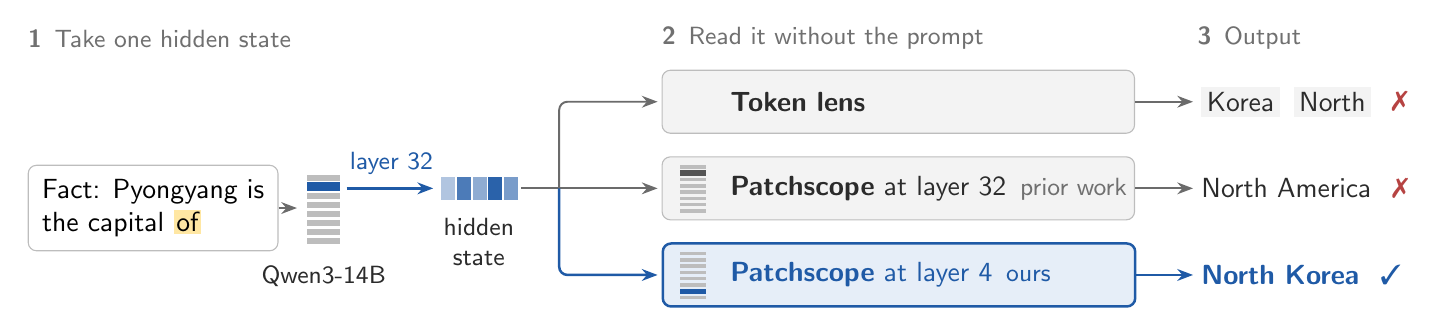
\begin{tikzpicture}[x=1cm,y=1cm]

% ---------------- column heads ----------------
\node[head] at (0.00,2.15) {\textbf{1}\enspace Take one hidden state};
\node[head] at (8.05,2.15) {\textbf{2}\enspace Read it without the prompt};
\node[head] at (14.85,2.15) {\textbf{3}\enspace Output};

% ---------------- source: prompt -> model -> one vector ----------------
\node[draw=line,rounded corners=3pt,fill=white,font=\normalsize,align=left,inner sep=5pt,anchor=west] (prompt) at (0.0,0.0)
  {Fact: Pyongyang is\\the capital {\setlength{\fboxsep}{1pt}\colorbox{tok}{of}}};

% the model as a stack of layers; read near the top (layer 32 of 40)
\stack{3.55,-0.46}{6}{ours}
\node[font=\small,text=ink,anchor=north] at (3.76,-0.62) {Qwen3-14B};
\draw[arr] (prompt.east) -- (3.42,0.0);
\draw[oarr] (4.05,0.25) -- (5.15,0.25);
\node[font=\small,text=ours,anchor=south] at (4.62,0.30) {layer 32};
\hvec{5.25,0.10}
\node[font=\small,text=ink,anchor=north,align=center] at (5.73,0.0) {hidden\\state};

% ---------------- fan-out to three readers ----------------
\coordinate (b) at (6.75,0.25);
\draw[line width=0.7pt,ink!70] (6.27,0.25) -- (b);
\draw[arr,rounded corners=3pt] (b) |- (8.0, 1.35);
\draw[arr] (b) -- (8.0,0.25) ;
\draw[oarr,rounded corners=3pt] (6.75,0.25) |- (8.0,-0.85);

% lane A: token lens
\node[lane,minimum width=6.0cm,anchor=west] (la) at (8.05,1.35) {};
\node[anchor=west,font=\normalsize,text=ink] at (8.80,1.35) {\textbf{Token lens}};
% lane B: Patchscope, same layer
\node[lane,minimum width=6.0cm,anchor=west] (lb) at (8.05,0.25) {};
\node[anchor=west,font=\normalsize,text=ink,align=left] at (8.80,0.25) {\textbf{Patchscope} at layer 32\enspace{\small\textcolor{mute}{prior work}}};
\minstack{8.28,-0.06}{6}{ink!80}
% lane C: Patchscope, early layer (ours)
\node[olane,minimum width=6.0cm,anchor=west] (lc) at (8.05,-0.85) {};
\node[anchor=west,font=\normalsize,text=ours,align=left] at (8.80,-0.85) {\textbf{Patchscope} at layer 4\enspace{\small ours}};
\minstack{8.28,-1.16}{1}{ours}

% ---------------- outputs ----------------
\draw[arr] (la.east) -- (14.80,1.35);
\draw[arr] (lb.east) -- (14.80,0.25);
\draw[oarr] (lc.east) -- (14.80,-0.85);

\node[outtext] (k) at (14.90,1.35) {\fboxsep=2pt\colorbox{soft}{Korea}\, \colorbox{soft}{North}};
\node[anchor=west,inner sep=0pt] at ($(k.east)+(0.25,0)$) {\cross};
\node[outtext] (na) at (14.90,0.25) {North America};
\node[anchor=west,inner sep=0pt] at ($(na.east)+(0.25,0)$) {\cross};
\node[outtext,text=ours] (nk) at (14.90,-0.85) {\textbf{North Korea}};
\node[anchor=west,inner sep=0pt] at ($(nk.east)+(0.25,0)$) {\tick};

\end{tikzpicture}
\end{document}
